% EACL 2027 anonymous review draft.
\documentclass[11pt]{article}
\usepackage[review]{acl}
\usepackage{times}
\usepackage{latexsym}
\usepackage[T1]{fontenc}
\usepackage[utf8]{inputenc}
\usepackage{microtype}
% Compatibility with the local Tectonic 2021 kernel; a current kernel defines this internally.
\makeatletter
\providecommand{\MT@maybe@textcmd}[1]{#1}
\makeatother
\usepackage{inconsolata}
\usepackage{graphicx}
\usepackage{amsmath,amssymb,array,booktabs}
% Generated by build_eacl_paper_results.py. Do not edit by hand.
\newcommand{\DelayPearson}{.318}
\newcommand{\DelaySpearman}{.347}
\newcommand{\DelayMSE}{.281}
\newcommand{\QualityPearson}{.435}
\newcommand{\QualityPearsonSD}{.037}
\newcommand{\QualitySpearman}{.463}
\newcommand{\QualitySpearmanSD}{.025}
\newcommand{\QualityMSE}{.259}
\newcommand{\QualityMSESD}{.012}
\newcommand{\QualityDelayPearson}{.475}
\newcommand{\QualityDelayPearsonSD}{.026}
\newcommand{\QualityDelaySpearman}{.515}
\newcommand{\QualityDelaySpearmanSD}{.016}
\newcommand{\QualityDelayMSE}{.246}
\newcommand{\QualityDelayMSESD}{.009}
\newcommand{\StructureDelayPearson}{.632}
\newcommand{\StructureDelaySpearman}{.618}
\newcommand{\StructureDelayMSE}{.187}
\newcommand{\FullPearson}{.658}
\newcommand{\FullPearsonSD}{.010}
\newcommand{\FullSpearman}{.652}
\newcommand{\FullSpearmanSD}{.007}
\newcommand{\FullMSE}{.177}
\newcommand{\FullMSESD}{.004}
\newcommand{\HumanPearson}{.809}
\newcommand{\HumanSpearman}{.707}
\newcommand{\HumanMSE}{.107}
\newcommand{\PrimaryDeltaPearson}{.1697}
\newcommand{\PrimaryPValue}{.000687}
\newcommand{\SecondaryDeltaPearson}{.030}
\newcommand{\SecondaryDeltaMSE}{-.012}
\newcommand{\CrossRtoR}{.909}
\newcommand{\CrossRtoS}{.430}
\newcommand{\CrossStoR}{.543}
\newcommand{\CrossStoS}{.552}
\newcommand{\LOIOQualityDelayPearson}{.377}
\newcommand{\LOIOQualityDelayPearsonSD}{.080}
\newcommand{\LOIOStructureDelayPearson}{.511}
\newcommand{\LOIOStructureDelayMacroPearson}{.332}
\newcommand{\LOIOFullPearson}{.573}
\newcommand{\LOIOFullPearsonSD}{.019}
\newcommand{\LOIODelayPearson}{.048}
\newcommand{\LOIODelayCenteredPearson}{.166}
\newcommand{\LOIODelayMacroPearson}{.173}
\newcommand{\LOIOQualityMacroPearson}{.229}
\newcommand{\LOIOQualityMacroPearsonSD}{.019}
\newcommand{\LOIOQualityDelayMacroPearson}{.221}
\newcommand{\LOIOQualityDelayMacroPearsonSD}{.024}
\newcommand{\LOIOFullCenteredPearson}{.340}
\newcommand{\LOIOFullCenteredPearsonSD}{.012}
\newcommand{\LOIOFullMacroPearson}{.358}
\newcommand{\LOIOFullMacroPearsonSD}{.005}
\newcommand{\InterraterExactPercent}{51.4}
\newcommand{\InterraterWithinOnePercent}{91.5}
\newcommand{\InterraterPearson}{.259}
\newcommand{\InterraterSpearman}{.261}
\newcommand{\InterraterICC}{.236}
\newcommand{\InterraterKappa}{.236}
\newcommand{\CohortN}{622}
\newcommand{\SpeechGroupN}{16}
\newcommand{\InterpreterN}{7}
\newcommand{\ZhEnN}{505}
\newcommand{\EnZhN}{117}
\newcommand{\BootstrapDraws}{10{,}000}
\newcommand{\PermutationCount}{65{,}536}
\newcommand{\RZeroCount}{19}
\newcommand{\ROneCount}{72}
\newcommand{\RTwoCount}{186}
\newcommand{\RThreeCount}{345}
\newcommand{\SZeroCount}{0}
\newcommand{\SOneCount}{33}
\newcommand{\STwoCount}{187}
\newcommand{\SThreeCount}{402}
\newcommand{\SourceUpperViolationMean}{55.3}
\newcommand{\SourceUpperViolationPercent}{8.9}
\newcommand{\SourceClippedPearson}{.482}
\newcommand{\SourceClippedPearsonSD}{.022}
\newcommand{\SourceClippedMSE}{.241}
\newcommand{\SourceClippedMSESD}{.007}
\newcommand{\SourceBoundedPearson}{.463}
\newcommand{\SourceBoundedPearsonSD}{.038}
\newcommand{\LOIOUpperViolationMean}{10.3}
\newcommand{\LOIOUpperViolationPercent}{1.7}
\newcommand{\LOIOClippedPearson}{.379}
\newcommand{\LOIOClippedPearsonSD}{.079}
\newcommand{\ResidualLQLow}{.200}
\newcommand{\ResidualLQHigh}{.246}
\newcommand{\ResidualEXPLow}{.114}
\newcommand{\ResidualEXPHigh}{.199}
\newcommand{\ResidualOnlyPearsonLow}{.091}
\newcommand{\ResidualOnlyPearsonHigh}{.197}
\newcommand{\ResidualPartialRLow}{.020}
\newcommand{\ResidualPartialRHigh}{.058}
\newcommand{\SecondaryDeltaPearsonCILow}{.002}
\newcommand{\SecondaryDeltaPearsonCIHigh}{.063}
\newcommand{\SecondaryDeltaMSECILow}{-.026}
\newcommand{\SecondaryDeltaMSECIHigh}{.000}
\newcommand{\QualityDelayPearsonCILow}{.381}
\newcommand{\QualityDelayPearsonCIHigh}{.596}
\newcommand{\QualityDelaySpearmanCILow}{.410}
\newcommand{\QualityDelaySpearmanCIHigh}{.642}
\newcommand{\QualityDelayMSECILow}{.188}
\newcommand{\QualityDelayMSECIHigh}{.314}
\newcommand{\QualityDelayMAECILow}{.335}
\newcommand{\QualityDelayMAECIHigh}{.431}
\newcommand{\QualityDelayMAE}{.382}
\newcommand{\PrimaryBootstrapDeltaPearson}{.157}
\newcommand{\PrimaryBootstrapDeltaSpearman}{.167}
\newcommand{\PrimaryBootstrapDeltaMSE}{-.035}
\newcommand{\PrimaryBootstrapDeltaMAE}{-.039}
\newcommand{\PrimaryBootstrapDeltaPearsonCILow}{.076}
\newcommand{\PrimaryBootstrapDeltaPearsonCIHigh}{.243}
\newcommand{\PrimaryBootstrapDeltaSpearmanCILow}{.086}
\newcommand{\PrimaryBootstrapDeltaSpearmanCIHigh}{.260}
\newcommand{\PrimaryBootstrapDeltaMSECILow}{-.075}
\newcommand{\PrimaryBootstrapDeltaMSECIHigh}{-.008}
\newcommand{\PrimaryBootstrapDeltaMAECILow}{-.071}
\newcommand{\PrimaryBootstrapDeltaMAECIHigh}{-.015}
\newcommand{\QualityAddedDelayDeltaPearson}{.040}
\newcommand{\QualityAddedDelayDeltaPearsonCILow}{.002}
\newcommand{\QualityAddedDelayDeltaPearsonCIHigh}{.066}
\newcommand{\SecondarySeedOneDeltaPearson}{.033}
\newcommand{\SecondarySeedOnePositiveGroups}{11}
\newcommand{\SecondarySeedOneValidGroups}{15}
\newcommand{\ResidualSeedOneDeltaPearsonCILow}{-.004}
\newcommand{\ResidualSeedOneDeltaPearsonCIHigh}{.071}
\newcommand{\SecondarySeedTwoDeltaPearson}{.030}
\newcommand{\SecondarySeedTwoPositiveGroups}{11}
\newcommand{\SecondarySeedTwoValidGroups}{15}
\newcommand{\ResidualSeedTwoDeltaPearsonCILow}{-.000}
\newcommand{\ResidualSeedTwoDeltaPearsonCIHigh}{.060}
\newcommand{\SecondarySeedThreeDeltaPearson}{.014}
\newcommand{\SecondarySeedThreePositiveGroups}{10}
\newcommand{\SecondarySeedThreeValidGroups}{15}
\newcommand{\ResidualSeedThreeDeltaPearsonCILow}{-.015}
\newcommand{\ResidualSeedThreeDeltaPearsonCIHigh}{.047}
\newcommand{\CrossRtoRCILow}{.855}
\newcommand{\CrossRtoRCIHigh}{.944}
\newcommand{\CrossRtoSCILow}{.348}
\newcommand{\CrossRtoSCIHigh}{.499}
\newcommand{\CrossStoRCILow}{.482}
\newcommand{\CrossStoRCIHigh}{.593}
\newcommand{\CrossStoSCILow}{.496}
\newcommand{\CrossStoSCIHigh}{.607}


\title{Predicting Professional Promptness Ratings in Simultaneous Interpreting from Text and Segment-Onset Delay}

\author{Anonymous EACL Submission}

\begin{document}
\maketitle

\begin{abstract}
Segment-onset delay is a natural timing signal in simultaneous interpreting, but it is not equivalent to a professional evaluator's judgment that an interpretation follows the source promptly. We formulate professional promptness-rating prediction as a supervised segment-level task using source text, interpreted output, and timing information. Our dataset contains \CohortN\ jointly rated Chinese--English and English--Chinese segments from \SpeechGroupN\ source-speech groups and \InterpreterN\ interpreters, evaluated for language quality (LQ), expressiveness (EXP), and promptness by two senior professional interpreters. We use their predefined two-rater professional aggregate, the equal-weight mean, while auditing evaluator-specific calibration. Under cross-fitted source-speech-group-held-out evaluation, segment-onset delay alone achieves Pearson $r=\DelayPearson$; predicted LQ and EXP combined with delay reach $r=\QualityDelayPearson\pm\QualityDelayPearsonSD$. A stronger deterministic lexical/structural-plus-delay baseline reaches $r=\StructureDelayPearson$, and the full model reaches $r=\FullPearson\pm\FullPearsonSD$, indicating a modest, heterogeneous complementary association from predicted quality beyond structure and timing. Human-label cross-rater analyses show positive but asymmetric transfer, indicating that the quality--promptness relationship is not confined to within-evaluator score coupling but remains evaluator-dependent. Interpreter-disjoint evaluation remains positive but heterogeneous. At camera-ready, we will release anonymized labels, delay records, rubric, fold manifests, and code subject to the study's governance constraints.

\end{abstract}

\section{Introduction}
Simultaneous interpreting (SI) requires an interpreter to listen, analyze, retain information, and produce another language under severe temporal constraints. Segment-onset delay is consequently a natural timing signal. It is distinct from ear--voice span (EVS), which requires an explicit choice of source--target linguistic anchors. Yet a temporal offset alone does not answer a different question faced by users and professional evaluators: does an interpretation \emph{feel} delayed? A short onset gap can coexist with omissions, broken delivery, or an interpreter who has stopped keeping up; conversely, a longer but fluent and complete segment may be judged less harshly.

This distinction creates an underexplored NLP evaluation problem. We ask whether a system can predict a professionally rated \emph{promptness score}: a reverse-oriented judgment for which a larger value means \emph{less} experienced delay. The answer matters for feedback systems and future SI assistants because it connects observable timing and text signals to the aspect of promptness identified in professional evaluation.

We use three scope distinctions throughout. At the \emph{task} level, the outcome is a professional promptness rating rather than elapsed delay or validated real-time perception. At the \emph{measurement} level, the protocol specifies an equal-weight aggregate target from two comparably qualified evaluators; cross-rater commonality remains evaluator-dependent. At the \emph{generalization} level, source-speech-group-held-out evaluation tests unseen source content, whereas interpreter-disjoint evaluation tests output from a held-out interpreter while allowing source-speech overlap.

We compare three deployable signal families: segment-onset delay, deterministic lexical/structural features from the source and interpreted output, and automatically predicted professional quality. A frozen shared encoder with two rubric-supervised quality outputs predicts LQ and EXP; a fold-local Ridge model combines these estimates with timing and optional structural features. In source-speech-group-held-out evaluation, the held-out group is excluded from upstream quality training and checkpoint selection; inner partitions provide cross-fitted quality predictions for promptness-model training. Interpreter-disjoint evaluation excludes every segment from the held-out interpreter throughout quality estimation and promptness-model training.

The results support a signal-decomposition account. The primary comparison asks whether professionally supervised quality signals contain information absent from onset timing; it does not establish the neural system as the strongest deployable text-based model. Deterministic lexical/structural+delay provides that stricter baseline, with predicted quality adding a smaller, seed-sensitive association. Under interpreter-disjoint evaluation, the full system reaches $r=\LOIOFullPearson\pm\LOIOFullPearsonSD$, with substantial variation across interpreters. Cross-rater analyses identify positive but asymmetric associations, and professional comments illustrate how evaluators describe low promptness ratings despite short onset delay.

Our contributions are:
\begin{itemize}
    \item We formulate a reverse-oriented professional promptness-rating task distinct from segment-onset delay and define an aggregate target with evaluator-specific analysis.
    \item We provide source-speech-group-held-out and interpreter-disjoint cross-fitting protocols that prevent outer-entity labels from entering upstream quality training, checkpoint selection, or second-stage promptness-model fitting.
    \item We decompose timing, text-derived structural features, and cross-fitted rubric-supervised quality under the same cohort, including a fold-safe residualized-quality audit.
    \item We quantify individual-rater agreement and cross-rater human-label transfer, finding cross-evaluator commonality alongside evaluator-specific calibration; anonymized labels, delay records, rubric, splits, and code are planned for camera-ready release.
\end{itemize}

\section{Related Work}
\paragraph{Timing in simultaneous translation and interpreting.}
EVS and related measures provide reproducible descriptions of temporal offset when source--target linguistic anchors are explicitly aligned; automated EVS work makes the alignment choice part of the measurement problem~\citep{guo2024manual}. EVS also varies with text-specific factors, interpreter-specific factors, and individual variation~\citep{janikowski2025evs}, alongside segmentation, reformulation, and production decisions central to cognitive accounts of SI~\citep{gile1995effort,seeber2011cognitive}. In simultaneous machine translation, wait-$k$ and prefix-to-prefix policies make latency controllable during generation~\citep{ma2019stacl}, and extensions to simultaneous speech translation analyze latency--quality trade-offs in end-to-end settings~\citep{ma2020simulst}. Average Token Delay (ATD) further argues that latency metrics should account for output duration, not only the start timing of partial translations~\citep{kano2023atd}. Our timing feature instead uses segment-onset delay: the archived onset difference for a paired source/interpreted segment, without word-level anchors or manual alignment validation. It serves as a baseline and input feature for predicting professional promptness ratings.

\paragraph{Cognitive accounts of SI.}
Gile's Effort Model characterizes SI as concurrent listening/analysis, production, and memory demands~\citep{gile1995effort}. Resource-allocation accounts further model how these demands interact under cognitive load~\citep{seeber2011cognitive,seeber2012cognitive}. Such accounts motivate the possibility that timing, fluency, and content quality co-vary in professional judgments. We test whether quality-associated signals help recover professional promptness labels on held-out speeches.

\paragraph{Automatic quality estimation.}
COMET introduced learned neural evaluation from source and translation representations~\citep{rei2020comet}; CometKiwi is a reference-free QE system from the WMT 2022 shared task~\citep{rei-etal-2022-cometkiwi}. Work on SI evaluation has also warned that standard MT metrics can miss interpretation-specific phenomena such as summarization, paraphrasing, disfluency, and segmentation~\citep{wein2024barriers}. In SI assessment, professional feedback can distinguish language quality, delivery/expressiveness, and promptness. We use a shared encoder with two rubric-supervised quality outputs for LQ and EXP from source text and interpreted output. The outputs remain correlated, and a one-factor sensitivity performs similarly; our experiment tests whether this quality representation complements segment-onset delay.

\paragraph{Rater-aware subjective-label modeling.}
Human labels may combine item difficulty with annotator expertise, severity, and systematic bias; interpreter-performance testing likewise documents rater severity/leniency with multifaceted Rasch analysis~\citep{han2015rater}. Crowd-label models estimate latent targets jointly with annotator reliability~\citep{whitehill2009whose,raykar2010learning}, while neural crowd layers learn annotator-specific transformations during representation learning~\citep{rodrigues2018deep}. These methods motivate evaluator-conditioned thresholds, ordinal likelihoods, and hierarchical calibration for promptness ratings. Our primary experiment uses the equal-weight aggregate target, and the rater audit characterizes evaluator-specific calibration around it.

\paragraph{Analytic professional assessment.}
Segment-level analytic assessment can preserve distinctions hidden by a single aggregate score~\citep{han2021reimagined}. This motivates our explicit rubric and our treatment of professional comments as post-hoc qualitative evidence rather than model features. Unlike work that evaluates an interpretation with an automatic metric alone, we evaluate whether automatically predicted professional quality dimensions can bridge to a separate professional promptness judgment.

\section{Task, Data, and Professional Rubric}
For segment $s$, let $y_s$ denote the \emph{professional promptness score} (LAT in the archived rubric): the reverse-oriented professional judgment where a larger score means that the interpreted output is perceived as \emph{less} delayed. Let $d_s$ be segment-onset delay in seconds, $q_s^{\mathrm{LQ}}$ and $q_s^{\mathrm{EXP}}$ be human quality labels, and $\hat q_s^{\mathrm{LQ}}$, $\hat q_s^{\mathrm{EXP}}$ be automatic estimates. We report Pearson correlation, Spearman correlation, and mean squared error (MSE) under source-speech-group-held-out evaluation and interpreter-disjoint evaluation. Thus, a positive correlation means that a model recovers a higher versus lower promptness score; it does not mean longer delay receives a higher score.

\subsection{Data and Timing}
The primary cohort contains \CohortN\ segments from \SpeechGroupN\ speech groups and \InterpreterN\ interpreters: \ZhEnN\ Chinese-to-English and \EnZhN\ English-to-Chinese. A speech group contains one source speech and all included interpretations of that speech; holding out a group therefore prevents source-content overlap between training and evaluation. Group sizes range from 11 to 106 segments (median 37.5). Although small by standard ML-benchmark scale, shared-label SI data with aligned source--output pairs, timing records, and multidimensional professional ratings are difficult and costly to construct; this is a high-cost expert-annotation setting rather than conventional text classification. Each analysis unit is the source/interpreted-output pair retained in the scoring archive and keyed by source file and original segment identifier. Segment-onset delay is the archived interpreted-segment audio onset minus paired source-segment audio onset.

The archive contains 679 segment identifiers with records from both primary evaluators. Of these, 632 have complete LQ, EXP, and promptness ratings from both evaluators and a numeric archived onset difference. The other 47 are outside this complete-case timing candidate set: 40 lack archived onset differences for both evaluators, and seven lack an R05 promptness rating. The primary analysis retains 622 of the 632 complete candidates whose recorded onset differences fall within $[0,20]$ s (mean 4.59, median 4.0). The remaining ten are excluded solely by the onset-range rule: eight are negative ($-95.295$ to $-1.149$ s), and two exceed 20 s (100 and 304.331 s). The archive does not preserve enough boundary provenance to assign an individual cause to these values. This range is an analysis filter, not a behavioral threshold. Descriptive bins are left-closed and right-open, except the final 10--20-second bin includes 20 seconds.

Two senior professional interpreter evaluators, each with more than ten years of professional experience, provide the primary ratings. They had comparable professional experience and equivalent roles. The two evaluators were recruited through a professional interpreting company and compensated at a rate of RMB 1,000 per hour for their professional evaluation work. Each evaluator uses integer anchors from 0 to 3 and rated the full shared cohort. Before formal analysis, the protocol specified their equal-weight mean as the aggregate target; neither evaluator was designated as more reliable, as a gold-standard rater, or as an adjudicator, and there was no third evaluator or adjudication stage. We call this the \emph{predefined two-rater professional aggregate}, or operational aggregate. Averaging produces the observed .5-point increments and .5--3.0 range. A provenance audit repaired a filename--identifier conflict before the corrected \CohortN-segment cohort and all reported analyses were regenerated. Promptness agreement is Pearson $.259$, Spearman $.261$, ICC$(2,1)=.236$, and quadratic-weighted kappa $.236$; exact agreement is 51.4\% and within-one-point agreement is 91.5\%.

\begin{table}[t]
\centering
\small
\caption{Primary shared-label cohort.}
\label{tab:cohort}
\begin{tabular}{>{\raggedright\arraybackslash}p{.58\columnwidth}>{\raggedright\arraybackslash}p{.31\columnwidth}}
\toprule
Property & Value \\
\midrule
Segments / speech groups / interpreters & \CohortN\ / \SpeechGroupN\ / \InterpreterN \\
Chinese$\rightarrow$English segments & \ZhEnN\ \\
English$\rightarrow$Chinese segments & \EnZhN\ \\
Mean LQ, EXP, promptness target range & 0.5--3.0 \\
Retained segment-onset delay & 0--20 s \\
Outer-test speech-group size & 11--106 \\
Delay-bin counts (0--2 / 2--4 / 4--6 / 6--10 / 10--20 s) & 82 / 202 / 151 / 138 / 49 \\
\bottomrule
\end{tabular}
\end{table}

\subsection{Professional Rubric and Protocol Record}
Evaluators used the same analytic rubric with integer anchors from 0 to 3, with higher values representing better performance; averaging the two ratings produces 0.5-point increments in the shared target. Table~\ref{tab:rubric} reproduces the assessment dimensions and score direction. LQ concerns what was conveyed and how well it was expressed in the target language; EXP concerns delivery; the promptness score concerns the evaluator's experienced promptness, not a timestamp threshold. Consequently, a segment can have a short measured onset gap but a low promptness score if the interpretation loses the source, and a longer gap need not receive the minimum score if delivery remains coherent.

\begin{table*}[t]
\centering
\small
\caption{Professional analytic rubric. Individual ratings use integer anchors 0--3; the shared mean target has .5-point increments. Full anchor criteria appear in Appendix~A.}
\label{tab:rubric}
\begin{tabular}{>{\raggedright\arraybackslash}p{.18\textwidth}>{\raggedright\arraybackslash}p{.48\textwidth}>{\raggedright\arraybackslash}p{.25\textwidth}}
\toprule
Dimension & Assessment focus & Direction of score \\
\midrule
Language quality (LQ) & Adequacy and accuracy of conveyed content, together with well-formed target-language expression. & Higher is more accurate, complete, and linguistically well formed. \\
Expressiveness (EXP) & Fluency, naturalness, and delivery of the interpretation. & Higher is more fluent and natural. \\
Professional promptness (LAT) & How promptly the interpretation is experienced as following the source; reverse-coded with respect to experienced delay. & Higher is perceived as less delayed. \\
\bottomrule
\end{tabular}
\end{table*}

The retained rubric specifies integer anchors $\{0,1,2,3\}$ and verbal criteria; half-point values arise only after averaging individual ratings. The scoring platform enforced the rubric rule LQ$=0\Rightarrow$EXP$=0$ and promptness$=0$, so these lower-bound values are not three independent judgments. Appendix~A gives the criteria, Appendix~B reports audit details, and Appendix~C illustrates two observed professional-comment cases.

Both evaluators received the same written rubric before formal scoring. They jointly discussed example cases and completed a pilot calibration exercise, including the instruction that promptness concerned how promptly the interpretation was experienced as following the source and should be distinguished from LQ and EXP. Formal scoring then proceeded independently: both evaluators rated every retained segment and could not see each other's scores.

Both used headphones. Segment order was randomized. For each segment, evaluators listened to synchronized source and interpretation audio while viewing the corresponding transcripts; replay was permitted, and calculated segment-onset delay values were never shown. Within an item, the numerical scoring order was fixed as LQ, then EXP, then promptness/LAT. Evaluators could revisit and revise earlier scores. Optional comments were entered only after all three numerical ratings and are used only for post-hoc qualitative analysis.

The shared written instructions, joint pilot calibration, standardized presentation, full-cohort coverage, and independent blinded scoring make unequal task exposure or direct score sharing implausible explanations for disagreement. Its persistence is therefore consistent with evaluator-specific calibration. The fixed LQ$\rightarrow$EXP$\rightarrow$promptness sequence, same-session scoring, and permitted revision leave possible halo and fixed-order anchoring effects. The archive preserves per-segment source and interpreted text, numeric onset differences, scores, and optional comments, but not boundary-construction and onset-detection procedures or a manually validated timing subset. We therefore treat segment-onset delay as an archived onset-difference feature.

\paragraph{Rater-aware sensitivity.} The Results section reports same-rater and cross-rater human-label prediction under the same held-out speech-group folds. Under the independent scoring protocol above, positive cross-rater association reflects transfer across evaluator score patterns rather than direct score sharing; its asymmetry motivates evaluator-specific calibration analysis.

\section{Quality-Associated Promptness Prediction}
\subsection{Segment-Onset Delay Signal}
The main timing feature uses a continuous piecewise-linear basis with knots at 2, 4, 6, and 10 seconds,
\begin{equation}
\begin{aligned}
\phi(d_s)={}&[d_s, (d_s-2)_+, (d_s-4)_+,\\
             &\phantom{[}(d_s-6)_+, (d_s-10)_+],
\end{aligned}
\end{equation}
where $(x)_+=\max(0,x)$. A dated protocol freeze records these knots before any model run reported in this study; available provenance does not establish that they preceded all inspection of the cohort. We therefore treat them as one fixed representation and compare linear, quadratic, log-delay, alternative-knot, quantile-knot, and binned sensitivities.

\subsection{Text-Derived Structural Features}
The deployable structural baseline uses source and interpreted-output lexical-unit counts, target/source length ratio, target punctuation and sentence-ending counts, target lexical diversity, a very-short-output indicator, and language direction. For Chinese, each CJK character is one lexical unit; for alphabetic text, each alphanumeric word is one unit. These features use no human score and are standardized inside each outer training fold. They test whether an apparent quality advantage is instead explained by output completeness, direction, or other readily observed properties of the interpreted output.

\subsection{Quality Signals}
The same-rubric human-quality reference uses $(q_s^{\mathrm{LQ}},q_s^{\mathrm{EXP}})$ and provides a related-rubric comparison unavailable to a deployed system. The automatic setting replaces it with $(\hat q_s^{\mathrm{LQ}},\hat q_s^{\mathrm{EXP}})$, where $\hat q_s=f_\theta(x_s)$ and $x_s$ is the ordered pair (source transcript, interpreted-output transcript). The frozen \texttt{Unbabel/wmt22-cometkiwi-da} backbone encodes the pair with the implementation tokenizer (512-token truncation, first-token pooling); two linear residual heads predict LQ and EXP. Official head-only runs use AdamW for ten fixed epochs (batch size 16) and fixed weighted MSE, variance, and correlation losses; checkpoint selection maximizes development LQ Pearson+EXP Pearson. The anonymous model card gives all weights, tokenizer fallback, architecture, and inference details.

Construction scripts trace generated alignment sets to source markdown and Whisper interpretation transcripts, but the normalized archive has no per-record record of transcription, punctuation, editing, or segmentation provenance across the full cohort. Tokenizer revision and token-length logs are also unavailable, so we do not reconstruct a truncation rate. The predictor consumes complete text pairs only and is post-hoc rather than streaming.

\subsection{Source-Speech-Group-Held-Out Evaluation}
For each held-out source-speech group $g$, all automatic predictions for $g$ come from an upstream quality model trained and selected only on other groups. Exact duplicate source-text--interpreted-output pairs from $g$ are removed from upstream train and development partitions. This protects the outer test group from quality-label leakage and tests transfer to unseen source content.

The second-stage promptness-training side is also cross-fitted. Within the remaining groups, four inner source-speech-group partitions generate out-of-fold $\hat q^{\mathrm{LQ}}$ and $\hat q^{\mathrm{EXP}}$ for every promptness-training row. A final outer-excluded quality model predicts group $g$. The second-stage Ridge regressor is trained on inner out-of-fold features and evaluated on the final outer prediction. Thus, no row's second-stage quality feature is produced by a model that used that row's LQ/EXP label.

The 16 outer folds and four inner partitions are deterministic greedy segment-count balances, with stable name tie-breaks and no direction/interpreter stratification. Each final fold holds one group out; inner held-out groups supply OOF predictions, and all seeds reuse the same manifest. Quality models run for fixed ten epochs without early stopping; checkpoint selection uses development LQ Pearson+EXP Pearson, while hyperparameters are fixed and outer-test labels are never used. Ridge scaling is fit on outer promptness-training rows only; PCA is diagnostic only. Outer test inputs are used solely to remove exact duplicate source--output pairs from upstream train/dev, never their labels. The manifest and row-count inventory are part of the planned camera-ready reproducibility release.

The full procedure is repeated for all 16 outer groups and the held-out predictions are concatenated before computing corpus-level metrics. The second-stage model is $\hat y_s=g_\beta([\hat q_s,\phi(d_s),\psi(x_s)])$, where $\psi$ denotes optional structural features. We compare $\phi(d)$ alone; structural features with delay; predicted LQ/EXP with delay; and their combination. Numeric features are standardized using only the promptness-training portion of each outer fold, and Ridge regularization is fixed at $\alpha=1.0$. Fixed-alpha sensitivity over OLS and $\alpha\in\{.01,.1,1,10,100\}$ is reported separately. The human row provides the same-rubric reference described above.

Because the target is bounded to $[.5,3.0]$ but Ridge is unbounded, we audit the primary predicted-quality-plus-delay system for each outer protocol and seed. We report counts below .5 and above 3.0, Pearson/Spearman, MSE, MAE, and calibration from the descriptive regression $y=a+b\hat y$. As sensitivity analyses, we post-hoc clip only the held-out prediction, $\mathrm{clip}(\hat y,.5,3.0)$, and fit a separate fold-local bounded continuous model $\hat y=.5+2.5\,\sigma(X\beta)$ with the same fixed $\ell_2$ penalty. The latter is fitted solely on each outer training fold; neither sensitivity uses outer-test labels. We also report the corresponding fold-training-mean predictor. These checks assess range and calibration robustness rather than select a new primary model.

\subsection{Interpreter-Disjoint Evaluation}
We additionally hold out each of the seven interpreters in turn. Every segment from the outer interpreter is excluded from quality training, development, checkpoint selection, and promptness-model training. Within the remaining interpreters, four inner speech-group partitions generate OOF predicted LQ/EXP for promptness-model training; a final interpreter-excluded quality model predicts the held-out interpreter. We compare delay-only, structural features with delay, predicted quality with delay, and their combination, with no interpreter identity or global-mean feature. Source speeches may still appear through other interpreters, so this protocol evaluates output from a held-out interpreter with possible source-content overlap; we report both pooled and interpreter-level behavior.

\subsection{Evaluator-Specific Construct Audit}
The rater analysis uses the same 16 source-speech-group outer folds but human labels rather than automatic quality predictions. For every ordered quality-rater--target-rater pair, the Ridge mapping is fitted directly on the outer-training groups using the stated rater's LQ/EXP and shared segment-onset-delay features as inputs and the stated target rater's professional promptness ratings as outcomes. The fitted mapping is then evaluated on the held-out group's inputs from that same quality rater and outcomes from that same target rater. Thus, R05-quality$\rightarrow$R06-promptness and R06-quality$\rightarrow$R05-promptness are distinct target-specific models; no held-out target labels enter fitting or scaling.

\begin{figure*}[t]
\centering
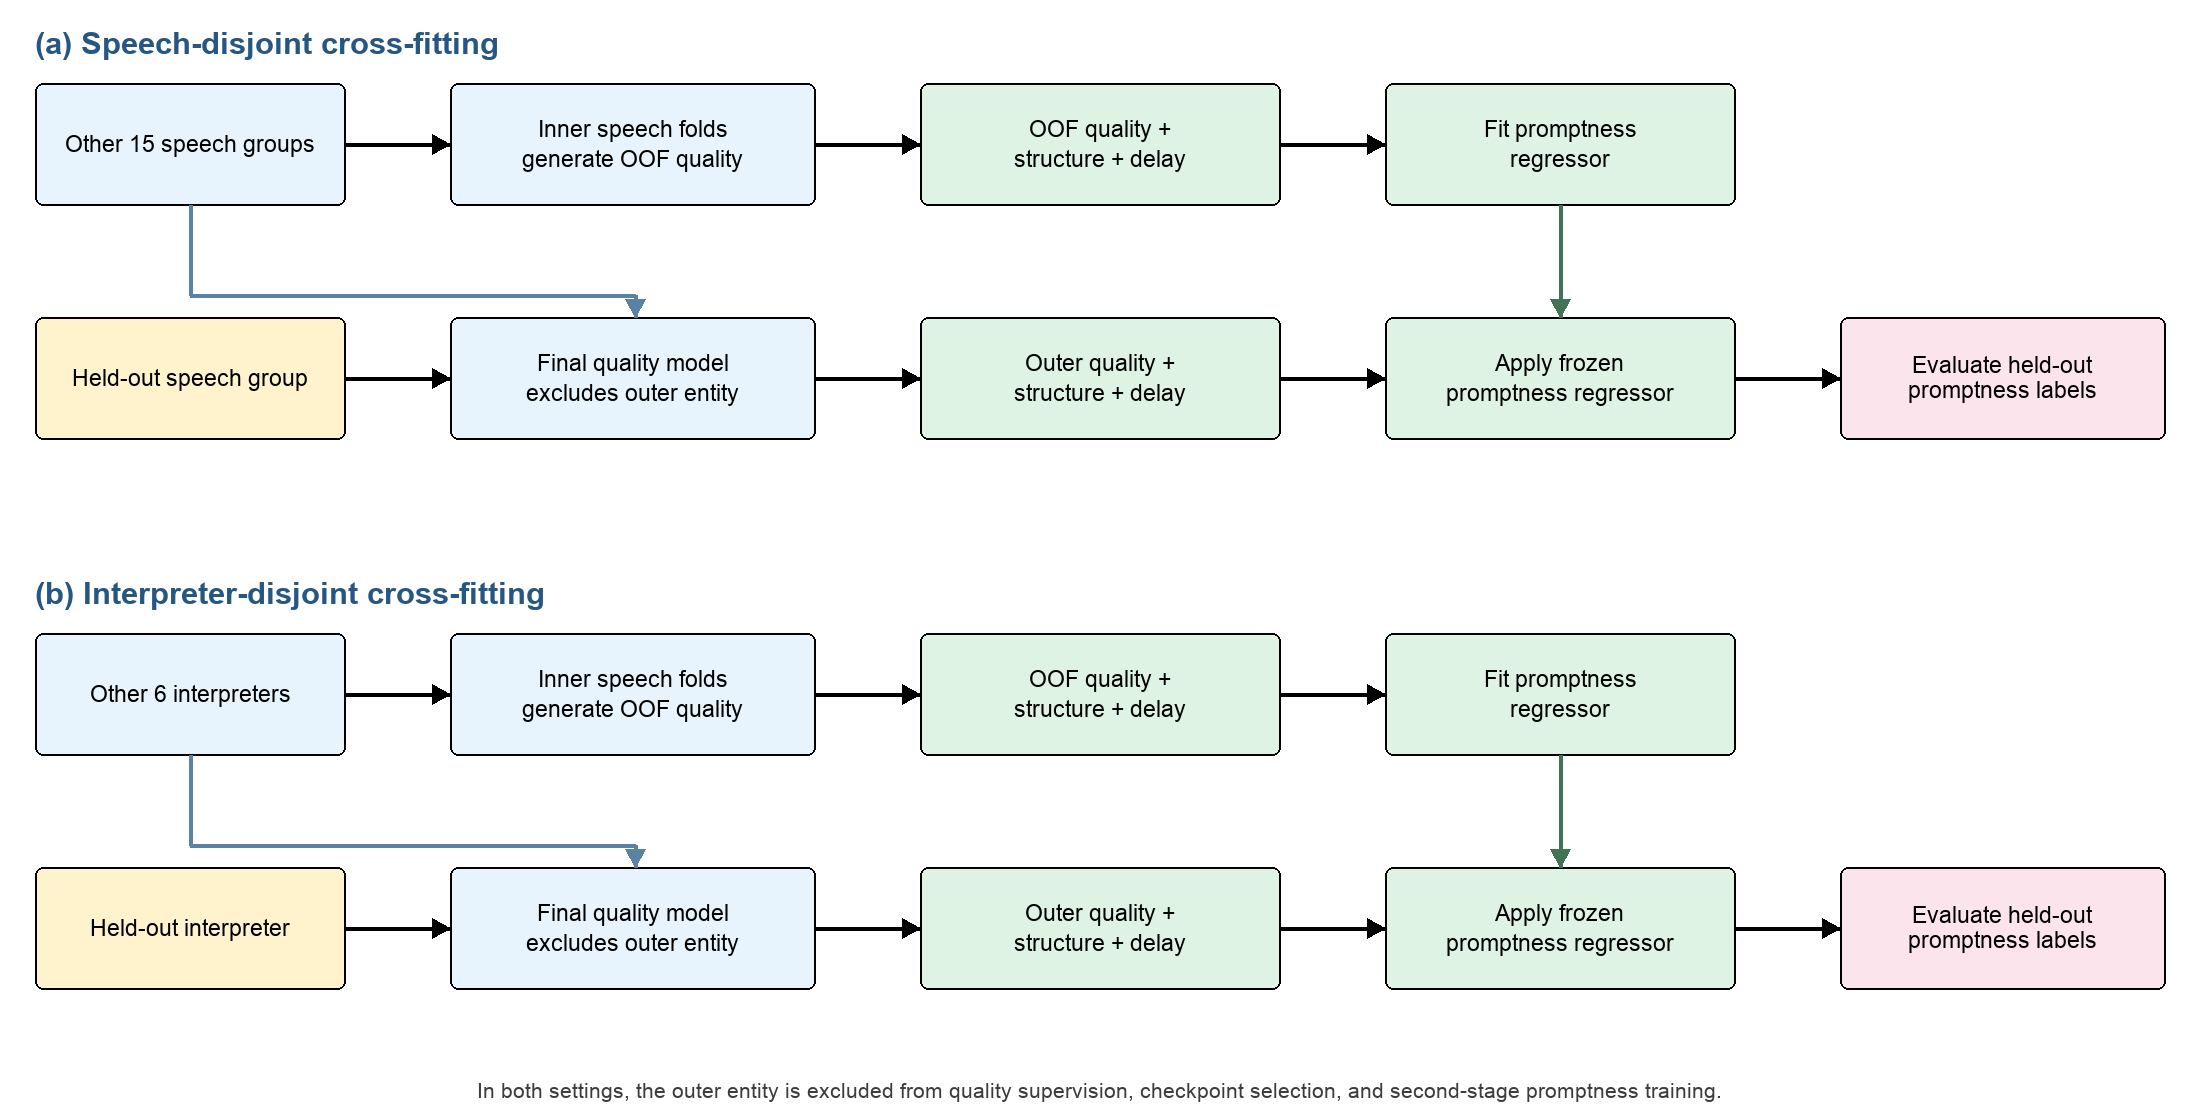
\includegraphics[width=.96\textwidth]{figures/fig_method_pipeline.png}
\caption{Cross-fitted two-stage protocols. Panel (a) holds out a speech group; panel (b) holds out an interpreter. In both settings the outer entity is excluded from quality supervision, checkpoint selection, and second-stage promptness-model training.}
\label{fig:pipeline}
\end{figure*}

\subsection{Uncertainty and Decision Rule}
Automatic point estimates are means over three fixed training seeds; their reported $\pm$ values are sample SDs across those seeds, not sampling confidence intervals. For source-speech-group-held-out results, we use 10,000 cluster-bootstrap draws: we resample the 16 source-speech groups with replacement, and each selected group contributes all of its segments. In every draw, we calculate each metric separately for each seed and then average it, matching the main-table point-estimate convention. The table delta averages seed-level correlations; the permutation uses segment-wise seed-mean predictions, so its system-level statistic differs because Pearson is nonlinear. We apply the identical group draw to paired systems to obtain CIs for their metric differences.

We define two comparisons. The \emph{primary prespecified comparison}, predicted quality+delay versus timing-only, tests the task's construct-level hypothesis that cross-fitted professional-quality signals add information beyond segment-onset delay. Its statistic is $T=r(y,\hat y_{Q+D})-r(y,\hat y_D)$. We enumerate all $2^{16}=65{,}536$ whole-group label swaps, preserve unequal observed group sizes in corpus correlation, use a two-sided alternative, and apply plus-one correction $p=(1+\#\{|T^*|\geq|T|\})/(1+65{,}536)$. The stricter secondary comparison, full versus structural+delay, asks whether predicted quality adds information beyond deterministic structure and timing. We report its paired cluster-bootstrap intervals and per-seed/group distributions descriptively, without another $p$-value. Seed-wise swaps and interpreter-disjoint results are descriptive. We report prediction SDs to detect collapse.

\section{Experiments and Analysis}
\subsection{Automatic Quality Prediction}
Across source-speech-group-held-out predictions, the two rubric-supervised outputs reach LQ Pearson $.450\pm.051$ and EXP $.415\pm.013$ across seeds, with raw-score SDs $.603$ and $.483$ (both above the .15 collapse diagnostic). Their high correlation ($r=.818$--$.894$) means that they form a non-collapsed, correlated quality representation rather than disentangled factors.

\begin{figure}[t]
\centering
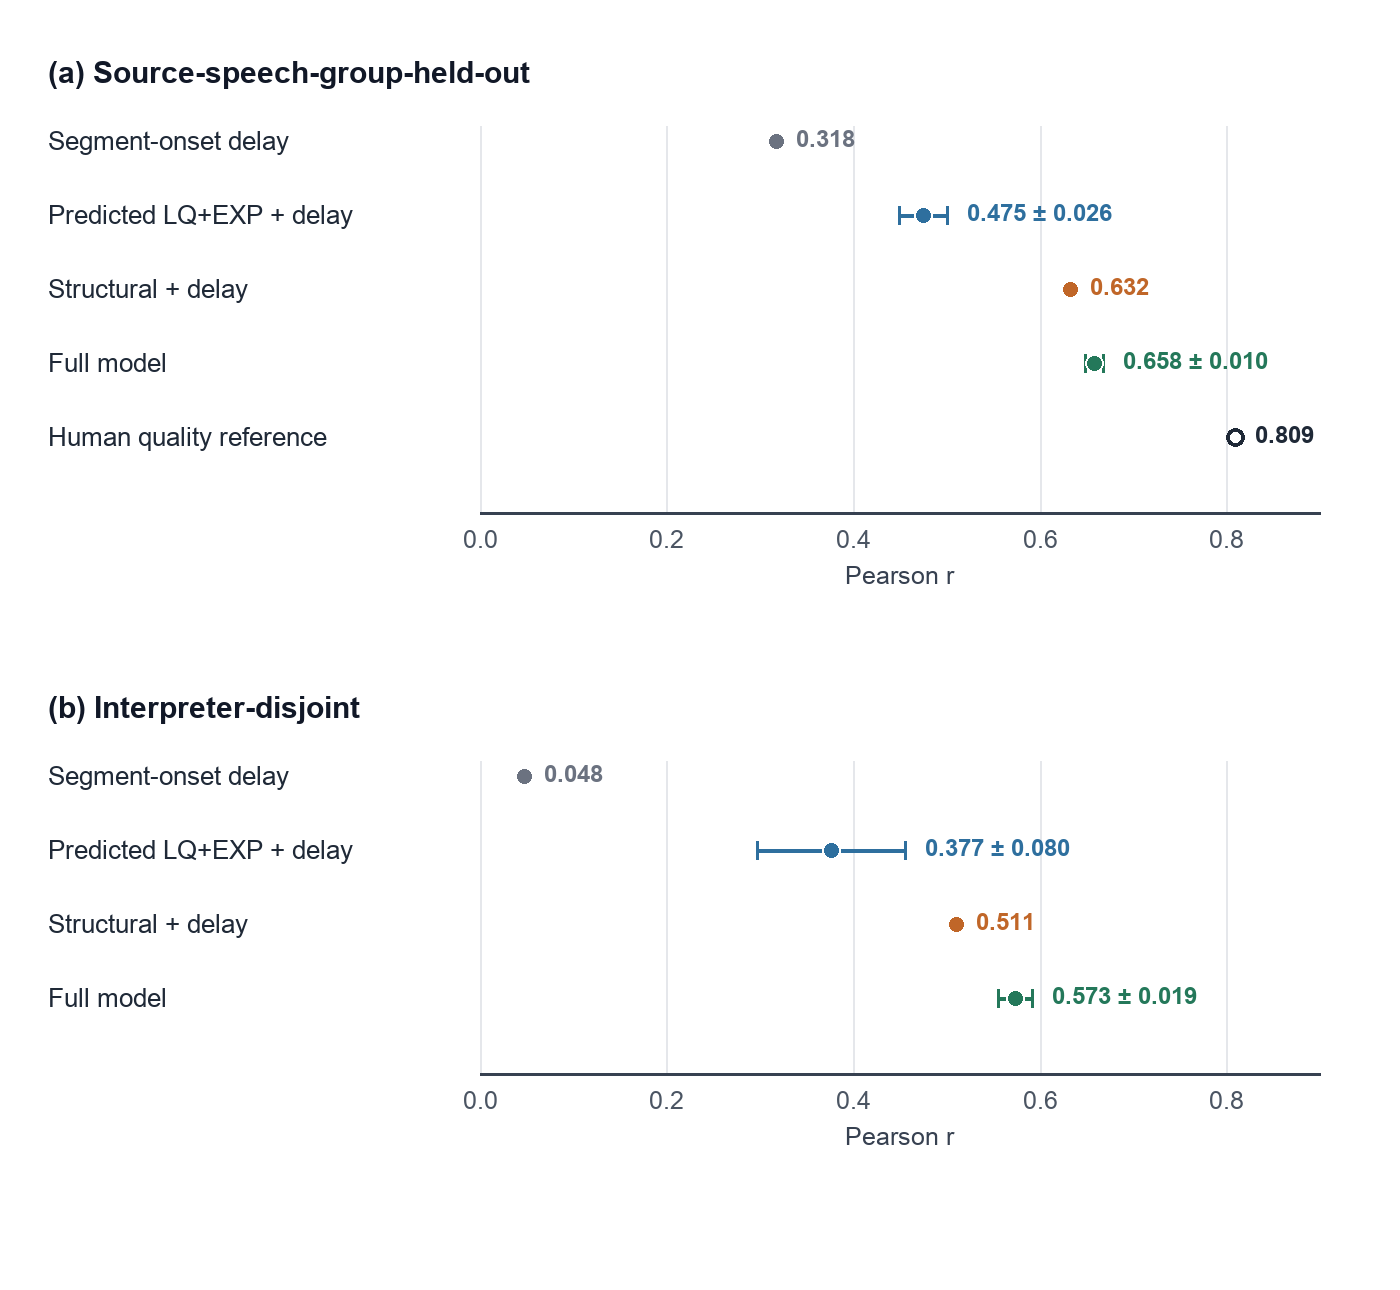
\includegraphics[width=.88\columnwidth]{figures/fig_main_model_comparison.png}
\caption{Main Pearson $r$ comparison. Automatic-row error bars are sample SD across three fixed seeds; clustered CIs appear in text. Deterministic systems appear once, and the hollow marker is the same-rubric human-quality reference.}
\label{fig:main-comparison}
\end{figure}

\subsection{Aggregate-Target Main Results}
\begin{table*}[t]
\centering
\scriptsize
\caption{Source-speech-group-held-out prediction of the predefined two-rater professional aggregate. Automatic rows are mean $\pm$ seed SD; the final row is the same-rubric human-quality reference.}
\label{tab:main}
\begin{tabular}{lccc}
\toprule
System & Pearson $r$ & Spearman $r_S$ & MSE \\
\midrule
Segment-onset delay only & \DelayPearson & \DelaySpearman & \DelayMSE \\
Predicted LQ+EXP & $\QualityPearson\pm\QualityPearsonSD$ & $\QualitySpearman\pm\QualitySpearmanSD$ & $\QualityMSE\pm\QualityMSESD$ \\
Predicted LQ+EXP + delay & $\QualityDelayPearson\pm\QualityDelayPearsonSD$ & $\QualityDelaySpearman\pm\QualityDelaySpearmanSD$ & $\QualityDelayMSE\pm\QualityDelayMSESD$ \\
Lexical/structural + delay & \StructureDelayPearson & \StructureDelaySpearman & \StructureDelayMSE \\
Predicted LQ+EXP + structural + delay & $\mathbf{\FullPearson\pm\FullPearsonSD}$ & $\mathbf{\FullSpearman\pm\FullSpearmanSD}$ & $\mathbf{\FullMSE\pm\FullMSESD}$ \\
\midrule
Same-rubric human-quality reference & \HumanPearson & \HumanSpearman & \HumanMSE \\
\bottomrule
\end{tabular}
\end{table*}

Table~\ref{tab:main} and Figure~\ref{fig:main-comparison} show that delay reaches $r=\DelayPearson$, predicted LQ+EXP $\QualityPearson\pm\QualityPearsonSD$, and predicted quality+delay $\QualityDelayPearson\pm\QualityDelayPearsonSD$. The primary prespecified comparison favors quality+delay over timing-only ($\Delta r=\PrimaryDeltaPearson$, two-sided exact whole-speech-group swap $p=\PrimaryPValue$) and addresses whether professionally supervised quality signals add information absent from onset timing. It does not establish the neural system as the strongest deployable text model: structural+delay reaches $\StructureDelayPearson$, while the full model reaches $\FullPearson\pm\FullPearsonSD$, with $\Delta r=\SecondaryDeltaPearson$ [$\SecondaryDeltaPearsonCILow,\SecondaryDeltaPearsonCIHigh$] and $\Delta\mathrm{MSE}=\SecondaryDeltaMSE$ [$\SecondaryDeltaMSECILow,\SecondaryDeltaMSECIHigh$]. Seed- and group-level effects are positive but heterogeneous; Appendix~B reports their distribution.

\paragraph{Speech-group-clustered uncertainty.} In \BootstrapDraws\ draws that resample the \SpeechGroupN\ speech groups with replacement and retain all segments in each selected group, quality+delay obtains $r=\QualityDelayPearson$ [$\QualityDelayPearsonCILow,\QualityDelayPearsonCIHigh$], $r_S=\QualityDelaySpearman$ [$\QualityDelaySpearmanCILow,\QualityDelaySpearmanCIHigh$], MSE $\QualityDelayMSE$ [$\QualityDelayMSECILow,\QualityDelayMSECIHigh$], and MAE $\QualityDelayMAE$ [$\QualityDelayMAECILow,\QualityDelayMAECIHigh$]. Relative to timing-only, $\Delta r=\PrimaryBootstrapDeltaPearson$ [$\PrimaryBootstrapDeltaPearsonCILow,\PrimaryBootstrapDeltaPearsonCIHigh$], $\Delta r_S=\PrimaryBootstrapDeltaSpearman$ [$\PrimaryBootstrapDeltaSpearmanCILow,\PrimaryBootstrapDeltaSpearmanCIHigh$], $\Delta$MSE $=\PrimaryBootstrapDeltaMSE$ [$\PrimaryBootstrapDeltaMSECILow,\PrimaryBootstrapDeltaMSECIHigh$], and $\Delta$MAE $=\PrimaryBootstrapDeltaMAE$ [$\PrimaryBootstrapDeltaMAECILow,\PrimaryBootstrapDeltaMAECIHigh$]. Its smaller gain over predicted quality is $\Delta r=\QualityAddedDelayDeltaPearson$ [$\QualityAddedDelayDeltaPearsonCILow,\QualityAddedDelayDeltaPearsonCIHigh$]. The $\pm$ values remain fixed-seed SDs.

\paragraph{Range sensitivity.} Raw quality+delay Ridge has no predictions below .5 and $\SourceUpperViolationMean/\CohortN$ ($\SourceUpperViolationPercent\%$) above 3.0. Clipping preserves performance ($r=\SourceClippedPearson\pm\SourceClippedPearsonSD$), while a fold-trained bounded model retains $r=\SourceBoundedPearson\pm\SourceBoundedPearsonSD$. Interpreter-disjoint clipping changes $r$ only from $\LOIOQualityDelayPearson\pm\LOIOQualityDelayPearsonSD$ to $\LOIOClippedPearson\pm\LOIOClippedPearsonSD$; Appendix~B reports full range, error, and calibration results.

\subsection{Structural-versus-Neural Signal Analysis}
Structural features explain limited variation in predicted quality (held-out $R^2=\ResidualLQLow$--$\ResidualLQHigh$ for LQ and $\ResidualEXPLow$--$\ResidualEXPHigh$ for EXP). Low structure-to-quality $R^2$ does not imply that raw quality contributes an orthogonal promptness signal: with both feature families in the linear second stage, residualization can preserve nearly the same joint prediction space. Residualized quality alone is weak ($r=\ResidualOnlyPearsonLow$--$\ResidualOnlyPearsonHigh$), promptness-residual prediction yields partial $R^2=\ResidualPartialRLow$--$\ResidualPartialRHigh$, and all seed-specific $\Delta r$ intervals cross zero. Accordingly, we interpret this comparison as a representation audit rather than an independent quality effect; Appendix~B gives details.

\subsection{Cross-Rater Analysis}
Using human LQ/EXP under the same held-out folds, R05 and R06 promptness ratings have Pearson $\InterraterPearson$ and ICC$(2,1)=\InterraterICC$; Appendix~B gives the full reliability audit.

With delay included, same-rater associations are $r=\CrossRtoR$ for R05 and $\CrossStoS$ for R06; cross-rater associations are $\CrossRtoS$ (R05 quality$\rightarrow$R06 promptness) and $\CrossStoR$ in reverse (Appendix Table~\ref{tab:cross-rater}). Under independent blinded scoring, these associations cannot arise from direct score sharing. They indicate cross-evaluator commonality in the quality--promptness relationship, but their asymmetry shows strong calibration dependence. Common rubric order and same-session scoring may still create parallel halo and anchoring effects.

\subsection{Interpreter-Disjoint Results}
After each interpreter is excluded, predicted quality+delay reaches pooled $r=\LOIOQualityDelayPearson\pm\LOIOQualityDelayPearsonSD$ versus \LOIODelayPearson\ for timing-only; structural+delay reaches \LOIOStructureDelayPearson\ and the full model $\LOIOFullPearson\pm\LOIOFullPearsonSD$ (Appendix Table~\ref{tab:loio}). The full model retains centered $r=\LOIOFullCenteredPearson\pm\LOIOFullCenteredPearsonSD$ and macro $r=\LOIOFullMacroPearson\pm\LOIOFullMacroPearsonSD$, but performance varies across interpreters. Source speeches may recur in this protocol.

\subsection{Direction Audit}
Direction-specific results are descriptive because the cohort contains 505 Chinese-to-English but only 117 English-to-Chinese segments. The full model is positive in both directions; Appendix Table~\ref{tab:automatic-direction} reports the automatic systems, and Appendix~B gives human-label sensitivity.

\section{Conclusion}
Professional promptness ratings are predictable from complementary timing, structural, and quality-associated signals under leakage-controlled evaluation. For unseen source speeches, predicted quality plus segment-onset delay improves over timing-only; structure is a stronger baseline, with a modest additional association from predicted quality. Interpreter-disjoint performance remains positive but heterogeneous. Cross-rater results indicate commonality in the quality--promptness relationship alongside evaluator-specific calibration. Future work should develop evaluator-conditioned and ordinal models under the same protocols.


% EACL main-content page boundary: the numbered paper ends within eight pages.
\clearpage
\section*{Limitations}
\paragraph{Task scope.} We predict deliberative professional promptness ratings collected with synchronized audio, visible transcripts, and permitted replay. The timing input is archived segment-onset delay; it has no manual alignment validation and should not be read as EVS, a causal threshold, or purely auditory real-time perception.

\paragraph{Measurement scope.} The aggregate target combines two comparably qualified, independently scoring evaluators without adjudication. Their shared rubric, pilot calibration, and standardized presentation reduce procedural differences, but available records do not establish whether pilot examples overlapped the analyzed cohort. The pilot preceded formal independent scoring and concerned rubric application rather than adjudicated final labels; any overlap could nevertheless reduce item-level rating independence. Fixed LQ$\rightarrow$EXP$\rightarrow$promptness order, same-session scoring, score revision, and the platform rule that LQ$=0$ forces the other two scores to 0 can strengthen low-end association; calibration does not establish evaluator-invariant validity.

\paragraph{Generalization scope.} Source-speech-group-held-out evaluation tests unseen source content. Interpreter-disjoint evaluation excludes one interpreter's output from training but allows source-speech overlap, and its subgroup results vary across interpreters. The language directions are imbalanced, and separate automatic rater-specific estimators remain future work.

\section*{Ethics Statement}
The study received approval from the relevant institutional review board, and all participating interpreters provided informed consent for use of their recordings and associated study data. Raw recordings, verbatim transcript pairs, and the interpreter-identity crosswalk are not publicly released because this seven-interpreter cohort carries re-identification risk. The planned camera-ready release is restricted to anonymized labels, delay records, rubric, fold manifests, code, and environment specifications; any released text pairs will be de-identified/redacted subject to governance conditions. The model is for research and formative feedback, not employment, certification, or ranking. Limited promptness agreement requires more evaluators, balanced directions, subgroup checks, and safeguards against optimizing for speed alone.

\section*{Data and Code Availability}
To preserve anonymous review, this submission does not provide an identifying repository link. Subject to the study's governance constraints, the camera-ready release will include anonymized professional labels, archived segment-onset-delay records, the retained rubric, deterministic fold manifests, experiment scripts, and environment specifications. It will not include raw recordings, verbatim transcript pairs, or the interpreter-identity crosswalk. Any released text pairs will be de-identified/redacted where required by the consent and governance conditions.


\bibliography{references}

\clearpage
\appendix
\section*{Appendix A: Retained Rubric Definition}

Two senior professional evaluators rated each retained segment on LQ, EXP, and
professional promptness (LAT in the archived rubric) using the same 0--3 integer-anchor rubric. Higher
promptness means the interpretation was experienced as \emph{less} delayed. The
aggregate target is their equal-weight mean, which produces .5-point increments.
Both evaluators rated the full cohort independently after shared written instructions,
example discussion, and a pilot calibration exercise; neither served as adjudicator.
The scoring platform enforced LQ$=0\Rightarrow$EXP$=0$ and promptness$=0$; such
lower-bound triples therefore reflect a rubric constraint rather than independent
dimension-level decisions.
Table~\ref{tab:retained-grid} reproduces the retained anchor criteria.

\begin{table}[h]
\centering
\scriptsize
\setlength{\tabcolsep}{2pt}
\caption{Retained segment-level rubric definition. Individual evaluators use the integer anchors 0--3; .5-point values occur only in the two-rater mean target.}
\label{tab:retained-grid}
\begin{tabular}{p{.25\columnwidth}p{.66\columnwidth}}
\toprule
Dimension & Criteria summary \\
\midrule
LQ & 3: meaning is preserved with no major omission or distortion. 2: some omissions or inaccuracies, but the main message remains intact. 1: major omissions or distortions, including misleading or reversed meaning. 0: meaning is largely absent, misleading, or reversed. \\
EXP & 3: fluent, idiomatic; minor errors only. 2: generally fluent with noticeable awkwardness/errors. 1: frequent disfluency/grammar issues affecting delivery. 0: breakdown-level disfluency impedes comprehension. \\
Promptness\newline (archived label: LAT) & 3: low perceived lag; well synchronized. 2: occasional lag; manageable. 1: frequent noticeable lag; disjointed flow. 0: severe persistent lag; difficult to follow. \\
\bottomrule
\end{tabular}
\setlength{\tabcolsep}{6pt}
\end{table}

\section*{Appendix B: Additional Audit Results}

\paragraph{Platform-rule audit.} Among the $2\times\CohortN=1{,}244$
individual evaluator--segment score triples in the retained cohort, 17 have
LQ$=0$. All 17 also have EXP$=0$ and promptness$=0$, with no violation of the
platform rule; all 17 were assigned by R05. Thus, 17 of the \CohortN\ aggregate
segments (2.7\%) contain one platform-constrained lower-bound triple.

\paragraph{Rater agreement.} On all \CohortN\ jointly rated segments, R05 assigned scores
$\{0,1,2,3\}$ with counts $(\RZeroCount,\ROneCount,\RTwoCount,\RThreeCount)$ and R06 with counts
$(\SZeroCount,\SOneCount,\STwoCount,\SThreeCount)$. The rows of Table~\ref{tab:rater-confusion} are R05 scores
and the columns are R06 scores. Exact agreement is \InterraterExactPercent\%; within-one-point
agreement is \InterraterWithinOnePercent\%; Pearson and Spearman correlations are \InterraterPearson\ and \InterraterSpearman;
ICC$(2,1)$ and quadratic-weighted kappa are \InterraterICC\ and \InterraterKappa.

% Generated by build_eacl_paper_results.py. Do not edit by hand.
\begin{table}[h]
\centering
\small
\caption{Promptness-score confusion matrix: R05 rows, R06 columns.}
\label{tab:rater-confusion}
\begin{tabular}{c|rrrr}
\toprule
R05 $\backslash$ R06 & 0 & 1 & 2 & 3 \\
\midrule
0 & 0 & 4 & 8 & 7 \\
1 & 0 & 3 & 41 & 28 \\
2 & 0 & 16 & 60 & 110 \\
3 & 0 & 10 & 78 & 257 \\
\bottomrule
\end{tabular}
\end{table}


\paragraph{Individual-rater human-label sensitivity.} Table~\ref{tab:rater-human}
reports selected held-out speech-group results using human LQ/EXP labels. These
are construct diagnostics rather than deployable automatic systems. R05's
same-rater reference is much higher than R06's, and each rater is differently
related to the onset signal, reinforcing the evaluator-calibration framing.

% Generated by build_eacl_paper_results.py. Do not edit by hand.
\begin{table*}[t]
\centering
\scriptsize
\caption{Individual-rater human-label audit. Models are fitted within the same outer speech-group folds; intervals are speech-group clustered 95\% CIs.}
\label{tab:rater-human}
\begin{tabular}{llccc}
\toprule
Target & System & Pearson $r$ & Spearman $r_S$ & MSE \\
\midrule
R05 & Delay & .106 [.014,.220] & .098 & .656 \\
R05 & Same-rater LQ+EXP+delay & .909 [.855,.944] & .836 & .113 \\
R05 & Structure+delay & .613 [.457,.691] & .546 & .406 \\
R05 & Full human reference & .911 [.859,.944] & .840 & .111 \\
R06 & Delay & .400 [.293,.488] & .403 & .293 \\
R06 & Same-rater LQ+EXP+delay & .552 [.496,.607] & .547 & .242 \\
R06 & Structure+delay & .442 [.373,.498] & .479 & .281 \\
R06 & Full human reference & .545 [.481,.610] & .552 & .245 \\
\bottomrule
\end{tabular}
\end{table*}


\paragraph{Cross-rater associations.} Table~\ref{tab:cross-rater} gives the
same-rater and cross-rater results summarized in Section~5.4.

\begin{table}[h]
\centering
\footnotesize
\caption{Human-label cross-rater audit under source-speech-group-held-out folds. Inputs are the stated rater's LQ/EXP plus segment-onset delay; brackets are speech-group-clustered 95\% CIs.}
\label{tab:cross-rater}
\begin{tabular}{lcc}
\toprule
Quality inputs & Promptness target & Pearson $r$ \\
\midrule
R05 & R05 & \CrossRtoR~[\CrossRtoRCILow, \CrossRtoRCIHigh] \\
R05 & R06 & \CrossRtoS~[\CrossRtoSCILow, \CrossRtoSCIHigh] \\
R06 & R05 & \CrossStoR~[\CrossStoRCILow, \CrossStoRCIHigh] \\
R06 & R06 & \CrossStoS~[\CrossStoSCILow, \CrossStoSCIHigh] \\
\bottomrule
\end{tabular}
\end{table}

\paragraph{Interpreter-disjoint results.} Table~\ref{tab:loio} reports the
pooled and macro-interpreter results summarized in Section~5.5.

\begin{table}[h]
\centering
\footnotesize
\caption{Interpreter-disjoint prediction of the aggregate target. Automatic rows report mean $\pm$ seed SD; macro $r$ equally weights held-out interpreters.}
\label{tab:loio}
\begin{tabular}{lrr}
\toprule
System & Pooled $r$ & Macro $r$ \\
\midrule
Delay & \LOIODelayPearson & \LOIODelayMacroPearson \\
Pred. Q + delay & $\LOIOQualityDelayPearson\pm\LOIOQualityDelayPearsonSD$ & $\LOIOQualityDelayMacroPearson\pm\LOIOQualityDelayMacroPearsonSD$ \\
Structure + delay & \LOIOStructureDelayPearson & \LOIOStructureDelayMacroPearson \\
Full model & $\mathbf{\LOIOFullPearson\pm\LOIOFullPearsonSD}$ & $\mathbf{\LOIOFullMacroPearson\pm\LOIOFullMacroPearsonSD}$ \\
\bottomrule
\end{tabular}
\end{table}

\paragraph{Direction-specific automatic systems.} Table~\ref{tab:automatic-direction}
reports the automatic-system sensitivity results summarized in Section~5.6.

% Generated by build_eacl_paper_results.py. Do not edit by hand.
\begin{table*}[t]
\centering
\scriptsize
\caption{Direction-specific results for the actual automatic systems. Seeded rows report mean $\pm$ sample SD across three fixed training seeds; deterministic rows are shown once. These descriptive subgroups are imbalanced and are not direction-level significance tests.}
\label{tab:automatic-direction}
\begin{tabular}{llccc}
\toprule
System & Direction ($n$) & Pearson $r$ & Spearman $r_S$ & MSE \\
\midrule
Segment-onset delay & Zh$\rightarrow$En (505) & .337 & .364 & .243 \\
Segment-onset delay & En$\rightarrow$Zh (117) & .319 & .305 & .446 \\
Predicted LQ+EXP + delay & Zh$\rightarrow$En (505) & $.414\pm.022$ & $.452\pm.013$ & $.235\pm.007$ \\
Predicted LQ+EXP + delay & En$\rightarrow$Zh (117) & $.717\pm.037$ & $.786\pm.012$ & $.295\pm.021$ \\
Lexical/structural + delay & Zh$\rightarrow$En (505) & .575 & .557 & .181 \\
Lexical/structural + delay & En$\rightarrow$Zh (117) & .749 & .790 & .211 \\
Full model & Zh$\rightarrow$En (505) & $.600\pm.013$ & $.592\pm.007$ & $.174\pm.004$ \\
Full model & En$\rightarrow$Zh (117) & $.777\pm.010$ & $.820\pm.006$ & $.192\pm.006$ \\
\bottomrule
\end{tabular}
\end{table*}


\paragraph{Structural residualization.} For each source-speech-group-held-out
fold and seed, a structure-to-predicted-quality mapping was fit on outer-training
rows only, then applied to form train/test quality residuals. Structural features
explain only a limited proportion of variation in the predicted quality outputs.
Because raw and residualized quality span closely related feature spaces when
structural features are retained, near-identical full-model predictions follow
from linear feature-space equivalence. Table~\ref{tab:residualization}
adds two less algebraically redundant checks: residualized-quality-only prediction,
and prediction of the structure+delay promptness residual from quality residuals.
The latter gives a small held-out partial $R^2$, while every seed-specific paired
$\Delta r$ interval crosses zero.

% Generated by build_eacl_paper_results.py. Do not edit by hand.
\begin{table*}[t]
\centering
\scriptsize
\caption{Fold-safe residualization representation audit. $R^2_Q$ gives structure-to-predicted-LQ/EXP held-out $R^2$; model cells report Pearson $r$/MSE. Partial $R^2$ is the held-out error reduction when quality residuals predict the structure+delay professional-promptness residual.}
\label{tab:residualization}
\begin{tabular}{lcccc}
\toprule
Seed & $R^2_Q$ LQ/EXP & Residual Q only & Residual augmentation & Partial $R^2$ \\
\midrule
20260718 & .200/.199 & .197/.305 & .664/.176 & .057 \\
20260719 & .246/.114 & .091/.319 & .659/.176 & .058 \\
20260720 & .215/.144 & .113/.315 & .645/.183 & .020 \\
\bottomrule
\end{tabular}
\end{table*}


\paragraph{Cross-rater result provenance.} The values in Table~\ref{tab:cross-rater}
use a literal target-specific specification: for each ordered pair, the stated
quality rater's LQ/EXP plus delay are used to fit the stated target rater's
promptness scores within the outer-training speech groups. Earlier working values
of $.502$ and $.828$ came from a different domain-swap analysis that fitted each
rater to that same rater's promptness and substituted the other rater's feature
scale and target only at held-out evaluation. They are therefore superseded and
are not comparable estimates of the cross-rater matrix reported here.

\paragraph{Direction-specific rater audit.} Table~\ref{tab:rater-direction}
reports the two most informative human-label systems by direction. The
English-to-Chinese condition contains only 117 segments, so these intervals are
descriptive rather than a direction-level model comparison.

% Generated by build_eacl_paper_results.py. Do not edit by hand.
\begin{table*}[t]
\centering
\scriptsize
\caption{Direction-specific human-label sensitivity. Brackets are speech-group clustered 95\% CIs.}
\label{tab:rater-direction}
\begin{tabular}{llrrr}
\toprule
Target & System & Direction ($n$) & Pearson $r$ & MSE \\
\midrule
R05 & LQ+EXP+delay & Zh$\rightarrow$En (505) & .895 [.814,.948] & .103 \\
R05 & LQ+EXP+delay & En$\rightarrow$Zh (117) & .929 [.860,.981] & .157 \\
R05 & Structure+delay & Zh$\rightarrow$En (505) & .508 [.262,.585] & .384 \\
R05 & Structure+delay & En$\rightarrow$Zh (117) & .740 [.663,.775] & .503 \\
R06 & LQ+EXP+delay & Zh$\rightarrow$En (505) & .537 [.466,.601] & .258 \\
R06 & LQ+EXP+delay & En$\rightarrow$Zh (117) & .641 [.464,.732] & .173 \\
R06 & Structure+delay & Zh$\rightarrow$En (505) & .428 [.342,.486] & .295 \\
R06 & Structure+delay & En$\rightarrow$Zh (117) & .466 [.372,.548] & .221 \\
\bottomrule
\end{tabular}
\end{table*}


\paragraph{Reproducibility inventory.} The camera-ready package will include the
corrected-data release tag and correction log, a table-to-file provenance map,
the exact outer and inner fold manifests, train/development/test counts,
environment versions, model-card configuration, calibration/range audit,
direction and per-interpreter tables, and the qualitative case-selection rule.
The present anonymous review version omits identifying links and restricted raw
media or identity mappings. The numerical source for the manuscript is the
canonical \texttt{paper\_results.json}, generated by
\texttt{build\_eacl\_paper\_results.py}; the cross-rater estimand correction is
documented in the reproducibility correction log.

\section*{Appendix C: Illustrative Cases}

Table~\ref{tab:case-pairs} gives one positive and one negative observed case.
They were selected post hoc under the documented purposive rule in the
documented case-selection rule; comments are translated and shortened, and are not
model inputs. They illustrate how evaluators articulated their ratings, but do not independently validate the promptness construct.

\begin{center}
\begin{minipage}{\columnwidth}
\centering
\scriptsize
\renewcommand{\arraystretch}{1.12}
\setlength{\tabcolsep}{2pt}
\captionof{table}{Observed professional-comment examples. These are illustrations, not additional rubric anchors or quantitative evidence.}
\label{tab:case-pairs}
\begin{tabular}{p{.14\columnwidth}p{.76\columnwidth}}
\toprule
Case & Observed example \\
\midrule
Positive & \textbf{Source:} An English conditional explains that many children in orphanages are not orphans, so ``orphanage'' is a euphemistic label. \newline \textbf{Interpreted output:} The Chinese output retains both the condition and conclusion. \newline \textbf{Scores:} Promptness $3.0$; predicted promptness $3.05$; segment-onset delay 2.00~s. \newline \textbf{Comment:} ``Fast, steady, complete, and idiomatic.'' \\
Negative & \textbf{Source:} An English segment states that a Mars trip requires an Earth--Mars alignment launch window. \newline \textbf{Interpreted output:} The Chinese output gives an incorrect distance and omits the launch-window condition. \newline \textbf{Scores:} Promptness $0.5$; predicted promptness $2.35$; segment-onset delay 2.44~s. \newline \textbf{Comment:} ``Limited information capture; unable to form complete sentences.'' \\
\bottomrule
\end{tabular}
\renewcommand{\arraystretch}{1}
\setlength{\tabcolsep}{6pt}
\end{minipage}
\end{center}

\section*{Appendix D: Quality Estimator Model Card}

The upstream estimator maps a complete ordered pair of source and
interpreted-output transcripts to two continuous quality outputs. It does not
use audio, delay, professional scores, rater/interpreter identity, or a
reference translation, and it is a post-hoc segment model rather than a
streaming system.

\begin{center}
\begin{minipage}{\columnwidth}
\centering
\scriptsize
\setlength{\tabcolsep}{2pt}
\captionof{table}{Configuration of the cross-fitted quality estimator used in the reported runs.}
\label{tab:model-card}
\begin{tabular}{p{.28\columnwidth}p{.63\columnwidth}}
\toprule
Item & Formal configuration \\
\midrule
Backbone & \texttt{Unbabel/wmt22-cometkiwi-da}; \texttt{unbabel-comet==2.2.4} loader \\
Input & Source as sequence A, interpreted output as sequence B; maximum 512 tokens; max-length padding and truncation \\
Tokenizer & Checkpoint tokenizer when available; otherwise \texttt{microsoft/infoxlm-large} \texttt{XLMRobertaTokenizer}. Logs do not preserve which branch or the checkpoint revision hash. \\
Representation & First-token (CLS) pooling; two independent linear residual heads added to fold-training LQ/EXP means \\
Trainable parameters & Two heads only. The instantiated LoRA adapters (rank 8, $\alpha=16$, dropout .1, query/value targets) and backbone remain frozen. \\
Optimization & AdamW; head LR $5\times10^{-4}$; weight decay .01; batch 16; 10 fixed epochs; no scheduler or early stopping; gradient norm .5; CUDA mixed precision when available \\
Selection and seeds & Maximum development Pearson(LQ)+Pearson(EXP); seeds 20260718, 20260719, and 20260720 \\
\bottomrule
\end{tabular}
\setlength{\tabcolsep}{6pt}
\end{minipage}
\end{center}

For batch predictions $\hat q_L,\hat q_E$ and targets $q_L,q_E$, training
minimizes
\begin{equation}
\begin{aligned}
\mathcal L={}&\mathrm{MSE}(\hat q_L,q_L)+1.7\,\mathrm{MSE}(\hat q_E,q_E)\\
&+0.2\,\mathcal L_{\mathrm{var}}\\
&+0.25[1-r(\hat q_L,q_L)]\\
&+0.25[1-r(\hat q_E,q_E)].
\end{aligned}
\end{equation}
The variance term matches prediction variance to target variance using a
rolling 64-example buffer and a .15 target-variance floor. These anti-collapse
weights were fixed across reported runs; the archive does not preserve a
separate search that selected them. Development labels are rounded to the
nearest .5 only in the historical validation routine, whose predictions are
clamped to $[-1,4]$ for checkpoint-selection correlations; raw exported quality
predictions are unchanged. Transcript production/editing provenance,
historical truncation counts, exact hardware, and per-fold training time are
not preserved.

\section*{Appendix E: Reproducibility Details}

\paragraph{Software environment.}
The recorded execution environment used Python 3.10. Project requirements
specify PyTorch $\geq2.0$, Transformers $\geq4.30,<5$, and scikit-learn
$\geq1.3$; the COMET loader is fixed to \texttt{unbabel-comet==2.2.4}.
Historical run logs do not preserve exact PyTorch, Transformers, or
scikit-learn patch versions, so the release environment will pin tested
versions rather than retrospectively asserting unrecorded ones.

\paragraph{Compute and training.}
The cross-fitted neural quality estimators were trained with CUDA mixed
precision when a GPU was available; Ridge models, metric aggregation,
bootstrap intervals, and permutation tests are CPU analyses. The archive does
not retain the exact GPU model or per-fold wall-clock time. The quality heads
use batch size 16, 10 fixed epochs, AdamW with learning rate
$5\times10^{-4}$ and weight decay .01, and the fixed loss in Appendix~D.
All reported automatic results use seeds 20260718, 20260719, and 20260720 and
the same deterministic fold manifest.

\paragraph{Resampling and testing.}
Source-speech uncertainty uses 10,000 bootstrap draws with RNG seed 20260726.
Each draw samples the 16 source-speech groups with replacement and includes all
segments of every selected group; paired systems use the same draw. The
primary comparison averages each segment's predictions across the three seeds,
then enumerates all $2^{16}=65{,}536$ whole-group swaps. It uses a two-sided
absolute-difference statistic and the plus-one correction described in
Section~4.

\paragraph{Planned release.}
Subject to data-use restrictions, the camera-ready reproducibility package will
include executable analysis scripts, the tested environment lock and
requirements files, corrected-data version and checksum, correction log,
table-to-file provenance map, exact outer/inner fold manifests, aggregate
predictions needed to regenerate reported tables, and build instructions.
Restricted audio, verbatim transcripts, identity mappings, row-level
interpreter outputs, and model checkpoints will not be distributed in the
anonymous review package.

\end{document}
